\documentclass[a4paper]{article}

%% Language and font encodings
\usepackage[english]{babel}
\usepackage[utf8x]{inputenc}
\usepackage{algorithm}
\usepackage[noend]{algpseudocode}
\usepackage{amsfonts}
\usepackage{caption}
\usepackage{subcaption}
\usepackage[T1]{fontenc}
\usepackage{cancel}
\usepackage{enumerate}
%% Sets page size and margins
\usepackage[a4paper,top=3cm,bottom=2cm,left=3cm,right=3cm,marginparwidth=1.75cm]{geometry}
\usepackage{minted}
\usemintedstyle{manni}
%% Useful packages
\usepackage{amsmath}
\newcommand\norm[1]{\left\lVert#1\right\rVert}
\usepackage{graphicx}
\setlength{\marginparwidth}{2cm}
\usepackage[colorinlistoftodos]{todonotes}
\usepackage[colorlinks=true, allcolors=blue]{hyperref}
\usepackage{fancybox}
\usepackage{tikz}
\usetikzlibrary{trees}
\usepackage{tcolorbox}
\tcbset{subtitle style={halign=center}}
\usepackage{multirow}
\usepackage{array}
\newcommand\MyBox[2]{
  \fbox{\lower0.75cm
    \vbox to 1.7cm{\vfil
      \hbox to 1.7cm{\hfil\parbox{1.4cm}{#1\\#2}\hfil}
      \vfil}%
  }%
}
\usepackage{tabularx}

\renewcommand{\baselinestretch}{1.2}
\makeatletter
\newcommand*{\rom}[1]{\expandafter\@slowromancap\romannumeral #1@}
\newcommand{\floor}[1]{\left\lfloor #1 \right\rfloor}
\newcommand{\ceil}[1]{\left\lceil #1 \right\rceil}
\newtheorem{theorem}{Theorem}
\newtheorem{lemma}[theorem]{Lemma}
\makeatother
\title{Homework 0}
% \title{Homework \rom{0}}
\author{Duo Zhang}


\begin{document}

\maketitle

\section*{Conceptual Questions}
\subsection*{1}
\textbf{Question:}

What is K-Means clustering? How is it different from Meanshift?\\
\textbf{Solution:}

K-means clustering is a kind of clustering method by giving $k$ initial centroids, and then find the Voronoi partition of the space. Then do the assignment step by assigning each data point a class by which Voronoi cell it locates in. The next step is updating step which is to recalculate the centroid position for each Voronoi cell by calculating the mean of all data points in this cell, and then update the Voronoi partition of the space. Repeat the assignment step and update step until converge.

Mean shift is very similar to the whole process of K means but KMeans is generally considered a s hard clustering method since every data point has a very clear class and each class has very clear boundaries with other classes. However, Mean shift is not doing the Voronoi partition but estimating a probability distribution which leads to relatively vague boundaries among clusters and for each data point, they only have one estimated probability to be in each cluster.
\subsection*{2}
\textbf{Question:}
	
What is softmax? Under what cases does softmax computation become unstable?

\textbf{Solution:}

Softmax is a kind of function which finally normalize a vector to be a discrete distribution and the probability for each entry is determined by its own quantity. The formulation is listed below:
\begin{align*}
    softmax(\mathbf{z})_{i}=\frac{e^{z_{i}}}{\sum_{j=1}^{K} e^{z_{j}}} \quad \text { for } i=1, \ldots, K \text { and } \mathbf{z}=\left(z_{1}, \ldots, z_{K}\right) \in \mathbb{R}^{K}
\end{align*}
However, because of the usage of exponential function, some times if the entry $\textbf{z}$ is extremely large, then there might be a numerically overflow for the computation which is very hazardous and dangerous.
\subsection*{3}
\textbf{Question:}

What is regularization in CNNs? Explain one common technique used for regularization.\\
\textbf{Solutions:}

The regularization in CNNs refers to all the methods that prevent CNNs from overfitting in the training process and give more capacity for the model to generalize to some unseen data for the model. One common technique for neural network training is Dropout technique. If dropout is implemented on one layer of the neural network, then this means the outputs of some cell in this layer is set to 0, which introduces a lot of noise into this model so that the neural network can hardly fit the training dataset as exact as possible, instead, the model tends to learn some more general features and information from the training dataset.

\subsection*{4}
\textbf{Question:}

What is a GAN? What does it mean for a GAN to ‘mode collapse’?\\
\textbf{Solution:}

GAN is the abbreviation of Generative Adversarial Network. GAN generally consists of two parts, a generator and a discriminator. The training process for GAN is kind of like a game between the generator and the discriminator. More specifically, the generator takes in a random noise, and then generate something that is a mimic of the distribution in the real training dataset and give it to the discriminator, and what the discriminator tries to do is to determine if the input is a mimic or is authentic which is from the training dataset. After competing with each other in the training process, eventually the generator would generate something that the discriminator can not even know if it's authentic or a fake, in other words, the result generated by the generator is as real as the training dataset.

However, sometimes training process of GAN can result in failure. For example, the generator can only generate something in a very limited range, say, identical output for all rounds or a small set of outputs. A generator should have been capable of generating a large variety of outputs but finally ends with singularity, and this is called "mode collapse".

\subsection*{5}
\textbf{Question:}

What are some common initialization methods for Convolution layers and Fully Connected layers in a CNN?\\
\textbf{Solution:}

The easiest way to initialize all the weights and bias for a neural network is random initialization by just giving all the weights some random numbers. Another one I know is called He initialization which takes the size and scale of the neural network into consideration by simply multiplying the random weights with a coefficient:
\begin{align*}
    \sqrt{\frac{2}{\operatorname{size}^{[l-1]}}}
\end{align*}
where $\operatorname{size}^{[l-1]}$ means the size of the previous layer.

\section*{Coding Challenges}
\subsection*{6. Optimizing a Function}
\textbf{Question:}

Create a function that can find an approximate minimum in a given vector function $f_n$ that takes an $n$\_dimension vector as an input and gives a scalar-valued output. Treat the function $f_n$ as a black box; you can query it but you do not have any other information about it (More specifically, you cannot take the gradient of this function).\\
\textbf{Solution:}

\href{https://colab.research.google.com/drive/1YZ73Dy30io64voNbD6G3seQ63Hi_LHGt?usp=sharing}{My Colab Solution.}

Particle Swarm algorithm is utilized here to find the minimum of the black-box function $f$. The basic idea is
\begin{enumerate}
    \item Randomly initializing a set of particles with random initial velocity.
    \item For each time step, each particle moves towards somewhere between the particle that is on the best position where the function value is a minimal in all particles and the best position of its own in all time steps while preserving its own momentum.
\end{enumerate}
Then the algorithm will repeat process 1 and 2 until convergence. If we formulate the process, it should be like:
\begin{enumerate}
    \item $x_{k+1}^{i}=x_{k}^{i}+v_{k+1}^{i} \Delta t$
    \item $v_{k+1}^{i}=w v_{k}^{i}+c_{1} r_{1} \frac{\left(p_{k}^{i}-x_{k}^{i}\right)}{\Delta t}+c_{2} r_{2} \frac{\left(p_{k}^{g}-x_{k}^{i}\right)}{\Delta t}$
\end{enumerate}
where $x_{k+1}^{i}$ and $v_{k+1}^{i}$ are the position and the velocity for particle $i$ on time step $k+1$ and the time step length is $\Delta t$, and where $w$ is the inertia of the particle which decides how much momentum that the user wants the particle to keep, $c_1$ and $c_2$ represent the self-confidence and the social confidence respectively, $p_{k}^{i}$ is particle $i$’s best position so far, $p_k^g$ is the swarm’s best particle position at iteration $k$ so that a direction deviation for the velocity can be defined by $c_{1} r_{1} \frac{\left(p_{k}^{i}-x_{k}^{i}\right)}{\Delta t}+c_{2} r_{2} \frac{\left(p_{k}^{g}-x_{k}^{i}\right)}{\Delta t}$ given some random numbers $r_1, r_2$ between $[0,1]$. For the test case $f(x)=w^T A w$ where $w = \frac{x}{\lVert x \rVert}$, the algorithm needs 40 rounds to satisfy a $10^{-10}$ tolerance on average.
\subsection*{7. Detecting Breast Cancer}
\textbf{Question:}

One interesting application of machine learning is in the area of medical diagnoses. Implement Neural Network in python to classify the data into Benign or Malignant for the Wisconsin Diagnostic Breast Cancer (WDBC) dataset. 

Create your model as a self-contained Google Colab notebook, and attach a link to your write-up. For your convenience, we have created an (incomplete) colab notebook here that you can copy and start working on.

Things to keep in mind: 
\begin{enumerate}
    \item How will you choose the features? 
    \item How will you train, validate, and test your model?
    \item How will you overcome overfitting?
\end{enumerate}
\textbf{Solution:}
\subsubsection*{Colab Notebook}
My Colab Notebooks link is \href{https://colab.research.google.com/drive/1pgkRWooWQiUSFWXuV75HSUtzRIowMycu?usp=sharing}{here}
\subsubsection*{Fill the Missing Values}
First, we can load the dataset into the notebook and check if all the values of all the attributes are valid. As expected, the values in the column of attribute "Bare Nuclei" are not all integers. Some of them are listed as "?" which means the value of this sample is missing. In order not to reduce the total amount of training samples while comparing with the number of all samples, the number of samples with missing value is quite large. Thus a random sampling is utilized to fill out all the missing values by giving each "?" a uniformly drew integer from 1-10. Then the distribution of all the attributes is shown in the following Figure\ref{1}:
\begin{figure}[H]
\centering
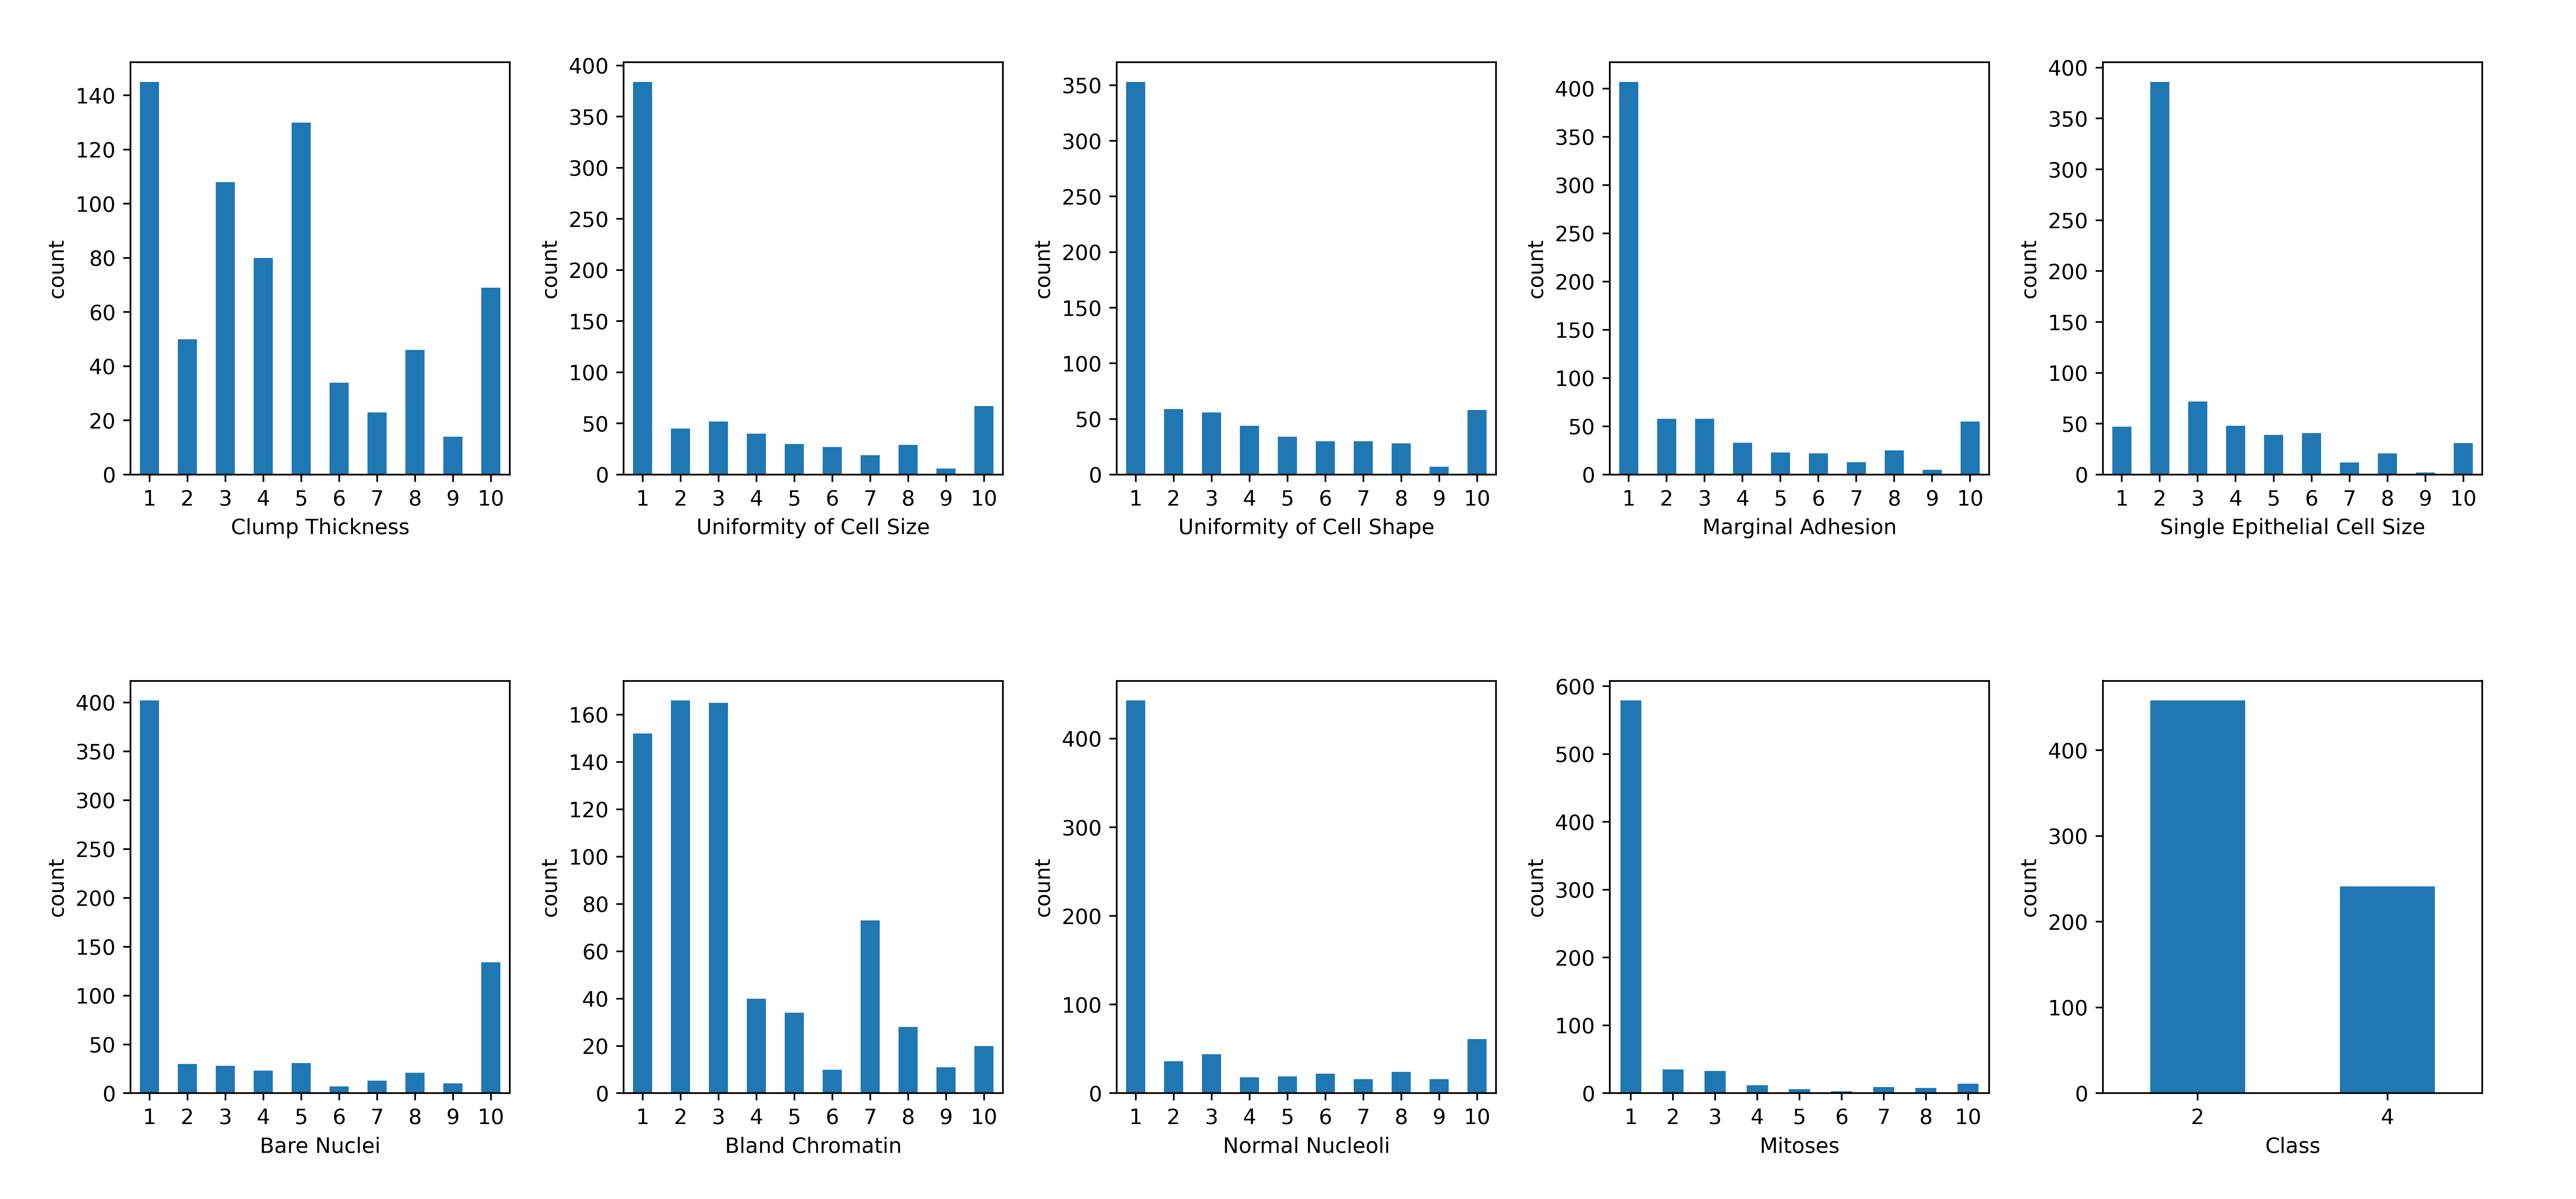
\includegraphics[width=1\textwidth]{all_attributes.png}
\caption{Distribution of attributes}
\label{1}
\end{figure}

As Figure\ref{1} implied, values of some attributes are very imbalanced. Therefore, feature selection can be implemented, but I will talk about feature selection later.
\subsubsection*{Normalization and Standardization}
The next thing is data preprocessing. For all the data without labels(denoted as $X$), they are first Min-Max Normalized and then Standardization. Afterwards, for convenience, the value set $\{\textit{2, 4}\}$ is replaced with $\{\textit{0, 1}\}$ where \textit{0} is for benign cases and \textit{1} is for malignant cases. 

\subsubsection*{Feature Selection}
To select proper features for the model to learn, the information gain for each attribute and the correlation between attributes and labels are calculated in Figure\ref{2} and Figure\ref{3}
\begin{figure}[h]
     \centering
     \begin{subfigure}[b]{0.45\textwidth}
         \centering
         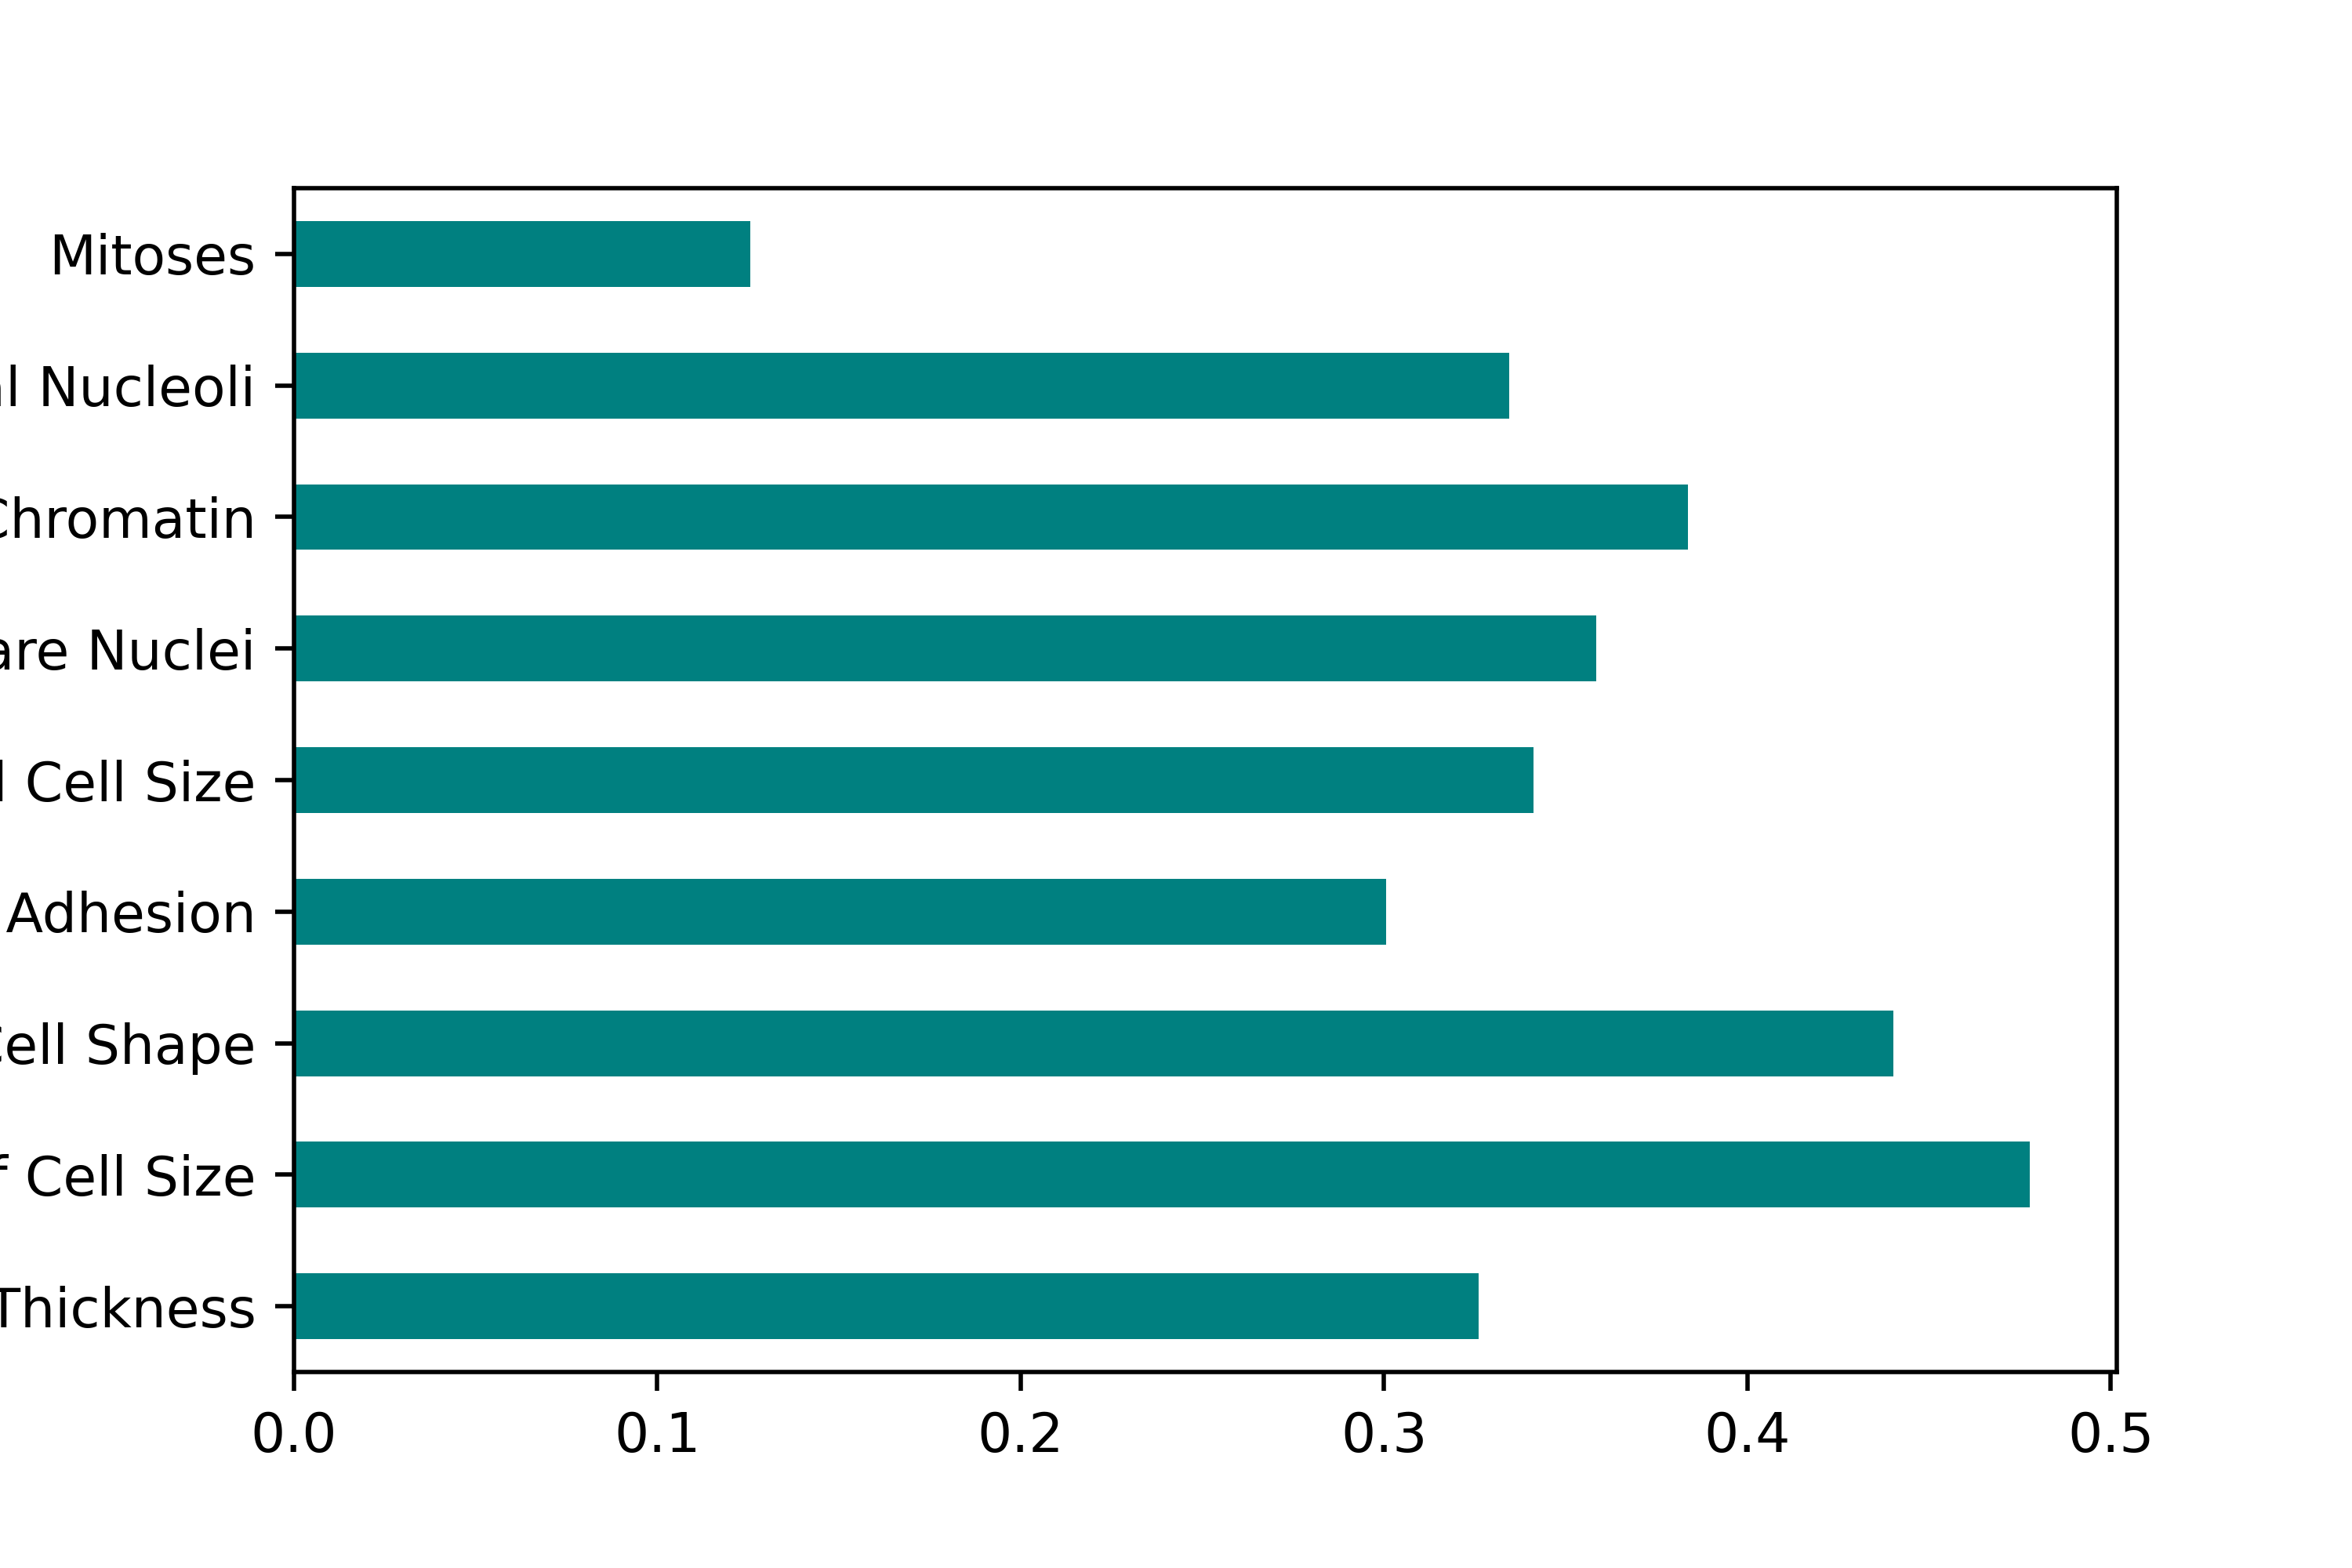
\includegraphics[width=\textwidth]{Information_gain.png}
         
         \caption{Information Gain for each attribute}
         \label{2}
     \end{subfigure}
     \hfill
     \begin{subfigure}[b]{0.45\textwidth}
         \centering
         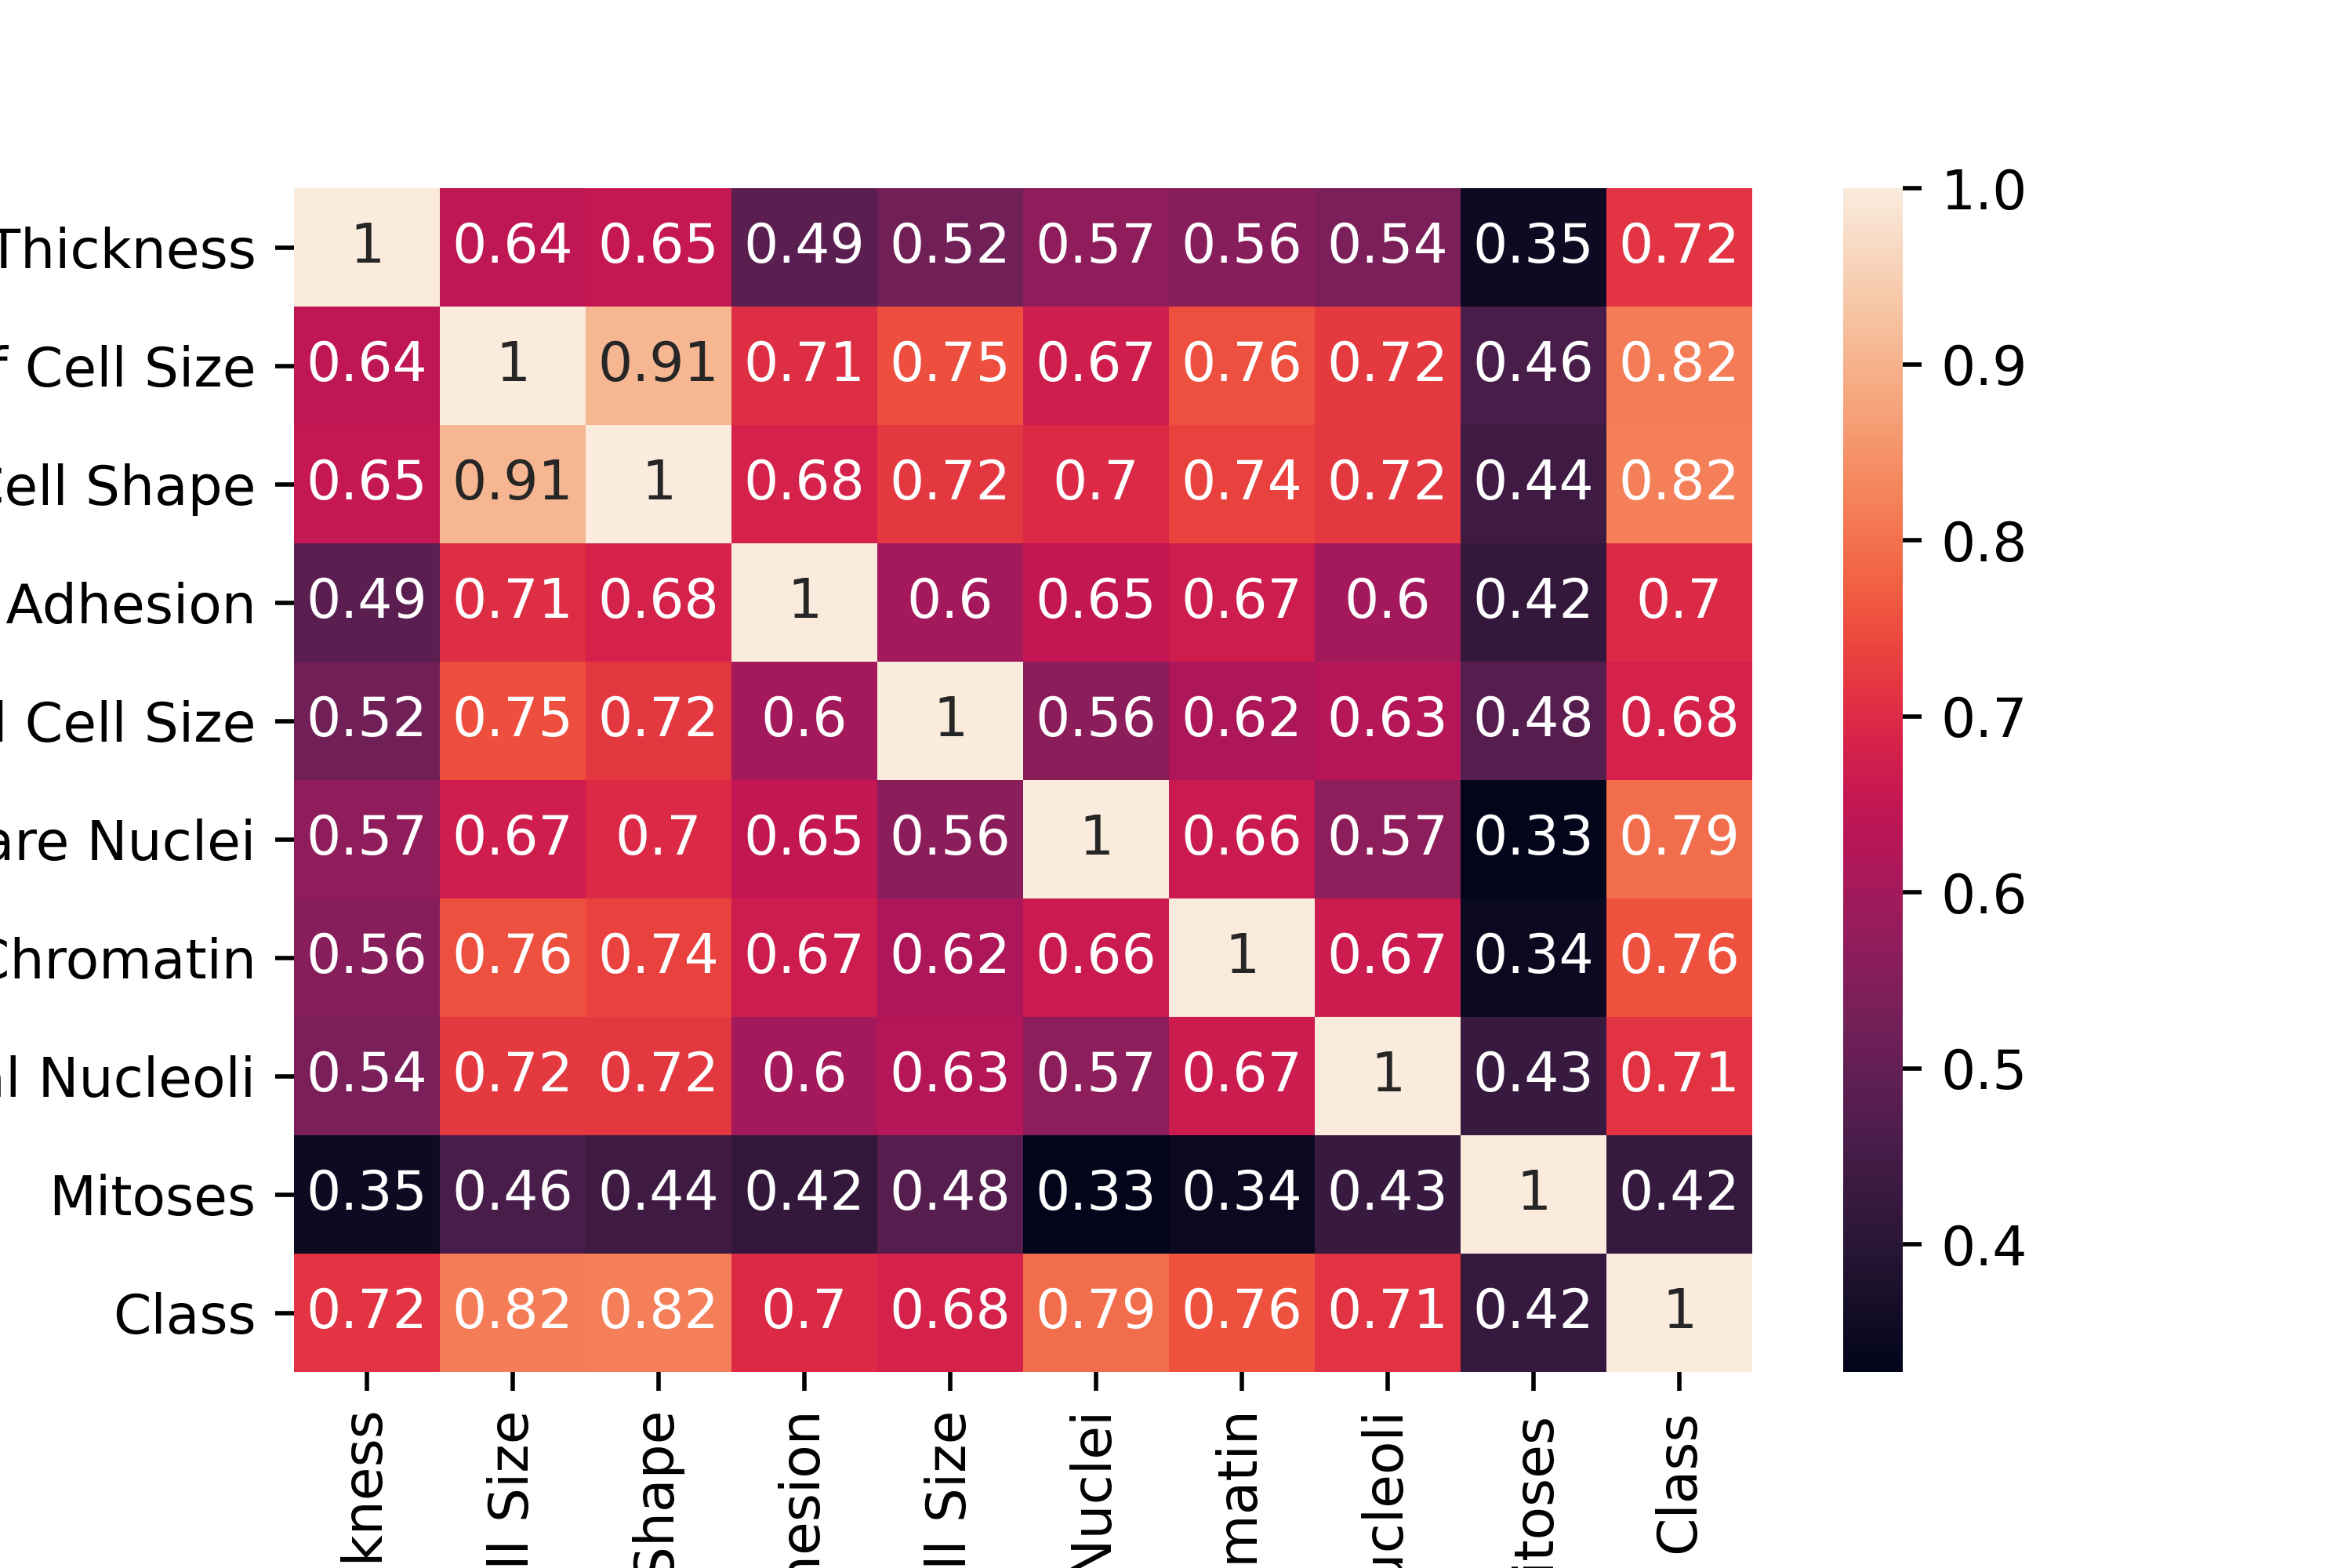
\includegraphics[width=\textwidth]{heatmap.png}
         \caption{Heat map of correlations of all attributes and labels}
         \label{3}
     \end{subfigure}
     \caption{}
\end{figure}
\subsubsection*{Split the Dataset}
I split the whole dataset into 3 parts: Training set, Validation set and Testing set with respective ratio 0.7, 0.1, 0.15.
\subsubsection*{Network Design}
The network is designed to be all dense linear layers including the input and output layers in which the number of hidden layers and the number of nodes in the hidden layer can be defined by user with torch.nn.ModuleList(), and dropout and batch normalization can be added by two switches.
\subsubsection*{Network Training, Validating and Testing}
While training, the total epoch is 200 and the training data is loaded with batch size 16 for each epoch. For every 10 epochs, the model is validated once. The model I choose has 3 hidden layers and 64 nodes for each layer. The information for the training process is listed below:
\begin{figure}[H]
\centering
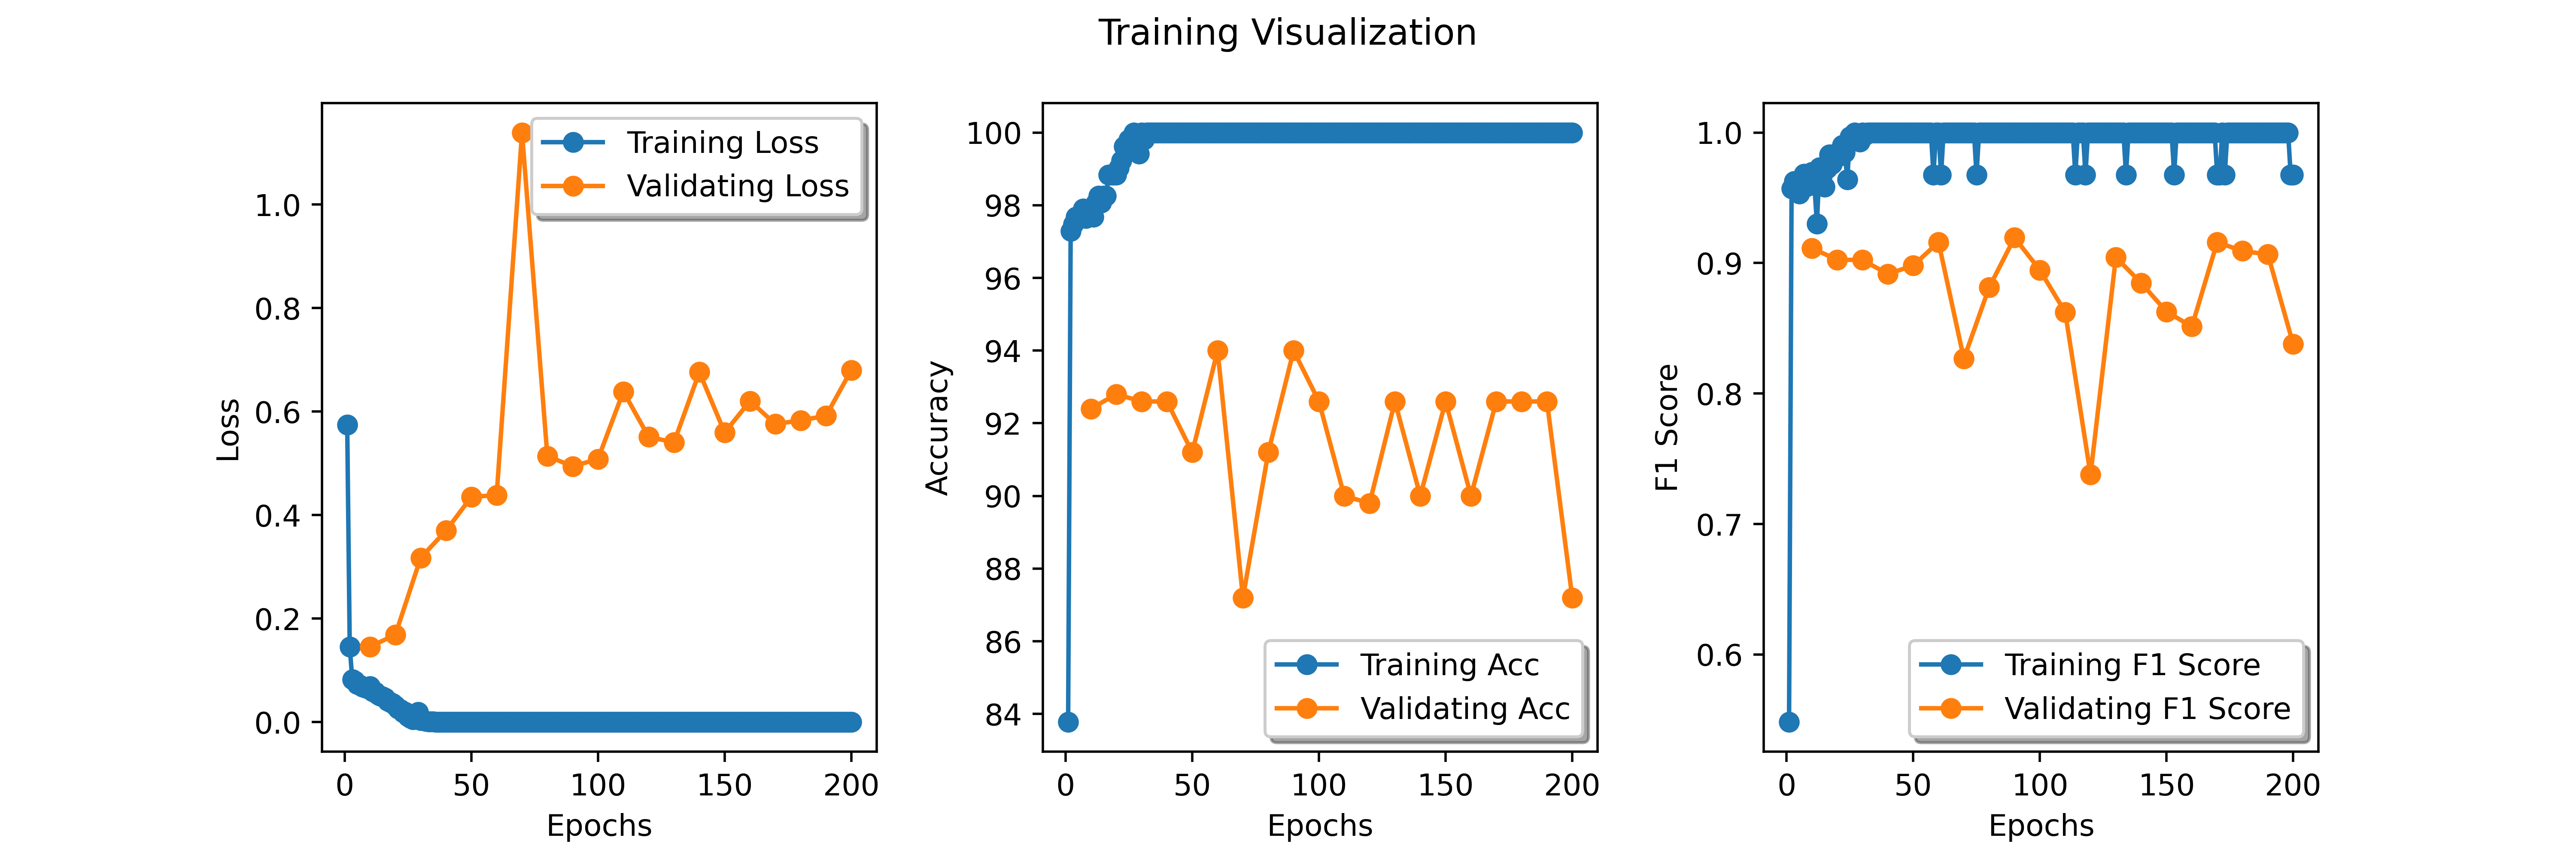
\includegraphics[width=1\textwidth]{64hn_3hl_200epochs_model.png}
\caption{Training Visualization for model with 3 hidden layers and 64 nodes for each hidden layer}
\label{4}
\end{figure}
Apparently according to the training and validation loss curve, this model is overfitting, but the validation f1 score and accuracy is not that bad. The test result is: 
\begin{center}
    \begin{tabularx}{1\textwidth}{| >{\centering\arraybackslash}X | >{\centering\arraybackslash}X|>{\centering\arraybackslash}X|>{\centering\arraybackslash}X|}
\hline
   Accuracy & Precision & Recall & F1 Score\\
   \hline
     95.333 & 0.9137931034482759 & 0.9636363636363636 & 0.9380530973451328\\
     \hline
\end{tabularx} 
\end{center}
The confusion matrix is (Confusion matrix is defined as Matrix\ref{def})
\renewcommand\arraystretch{1.5}
\setlength\tabcolsep{0pt}

\begin{table}
\begin{center}
    \begin{tabular}{c >{\bfseries}r @{\hspace{0.7em}}c @{\hspace{0.4em}}c @{\hspace{0.7em}}l}
  \multirow{10}{*}{\parbox{1.1cm}{\bfseries\raggedleft actual\\ value}} & 
    & \multicolumn{2}{c}{\bfseries Prediction outcome} & \\
  & & \bfseries p & \bfseries n & \bfseries total \\
  & p$'$ & \MyBox{True}{Positive} & \MyBox{False}{Negative} & P$'$ \\[2.4em]
  & n$'$ & \MyBox{False}{Positive} & \MyBox{True}{Negative} & N$'$ \\
  & \bfseries total & P & N &
\end{tabular}
\end{center}
\caption{Confusion Matrix}
  \label{def}
\end{table}


\begin{center}
    \begin{tabular}{|c|c|}
    \hline
    True Positive & False Negative \\\hline
        53 & 2 \\\hline
        5  & 81\\\hline
        False Positive & True Negative\\\hline
    \end{tabular}
\end{center}
Since the model is overfitting, maybe we can add drop out mechanism into the networks. Therefore, Dropout is added for each hidden layer with probability of 0.5. The training process is visualized in Figure\ref{5}:\\
\begin{figure}[h]
\centering
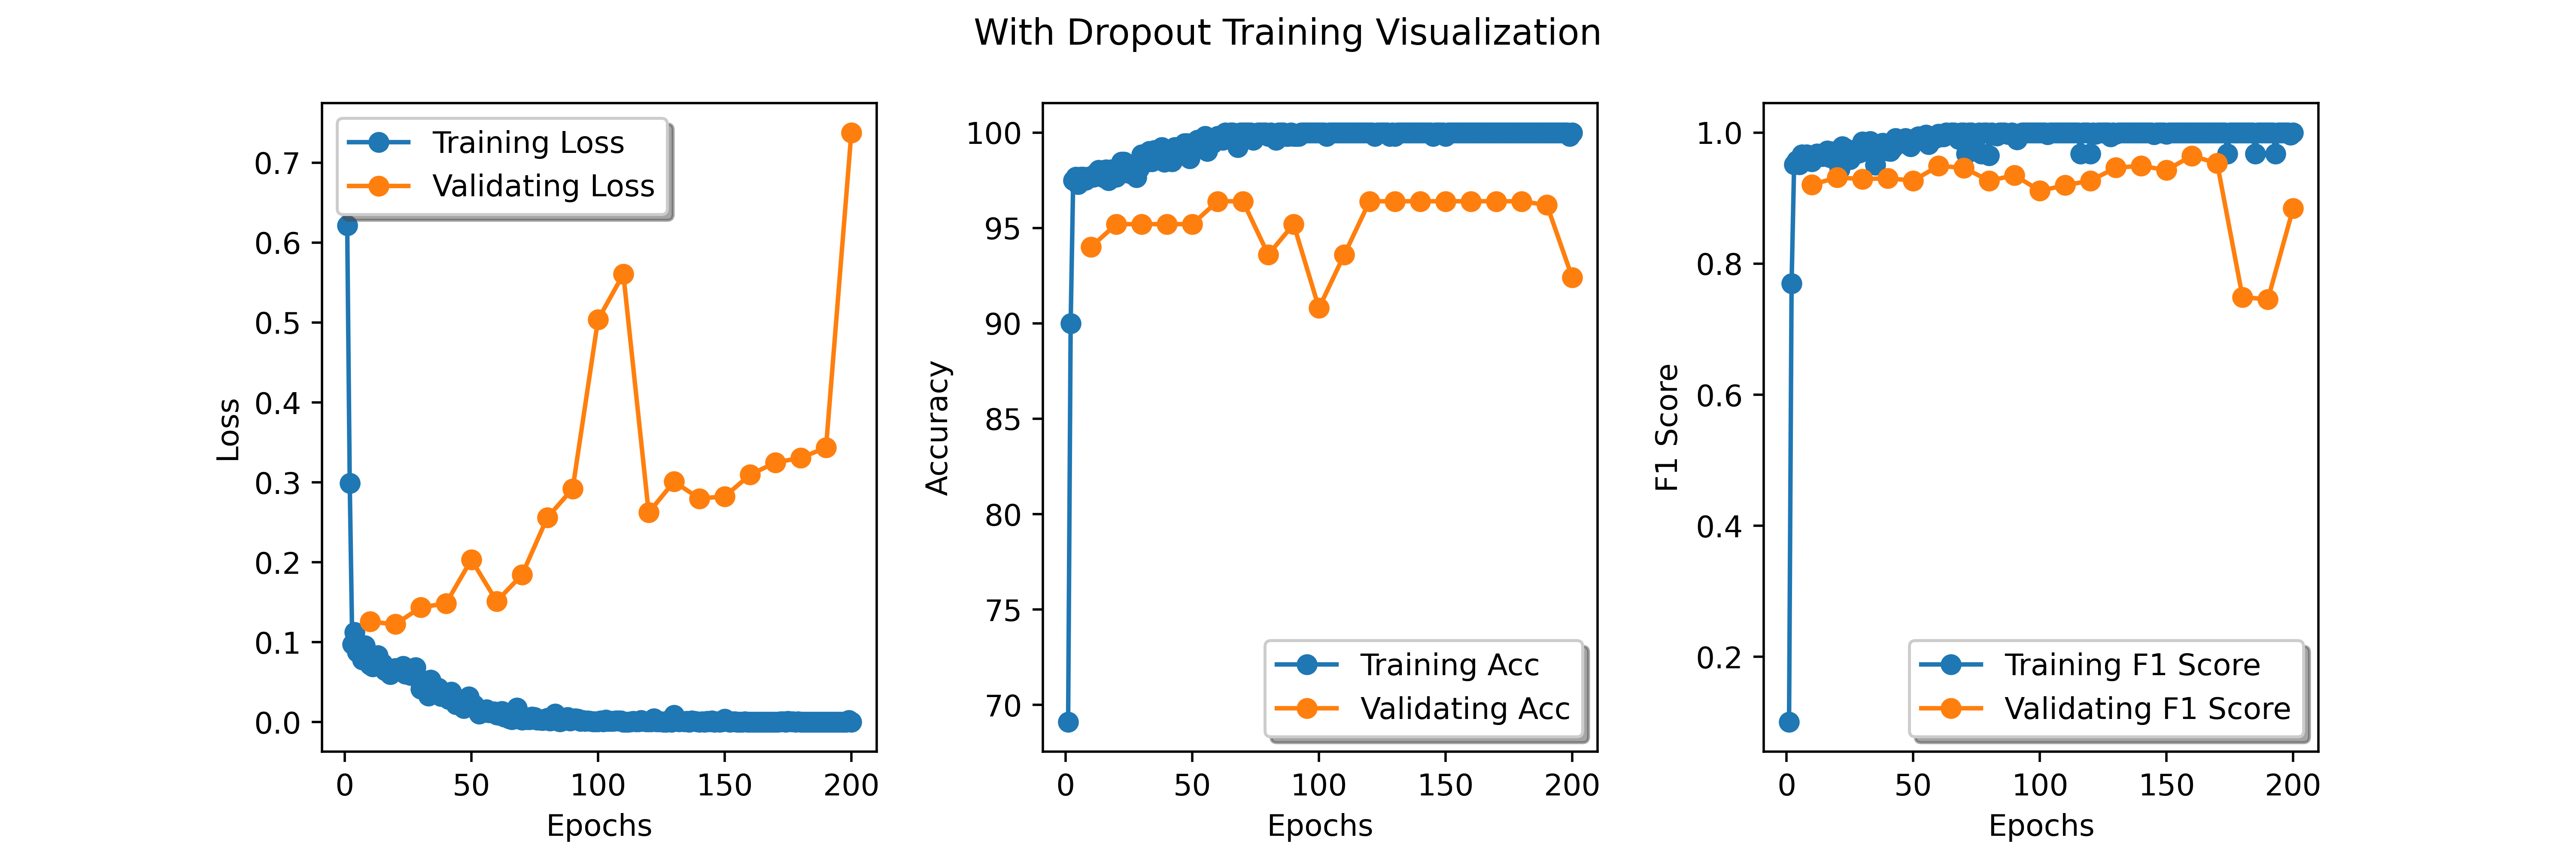
\includegraphics[width=1\textwidth]{Dropout_64hn_3hl_200epochs_model.png}
\caption{Training Visualization for model with 3 hidden layers and 64 nodes for each hidden layer with Dropout}
\label{5}
\end{figure}

As we can see, although the model is still overfitting, the accuracy and F1 score tends to be better. The test result is:

\begin{center}
   \begin{tabularx}{1\textwidth}{| >{\centering\arraybackslash}X | >{\centering\arraybackslash}X|>{\centering\arraybackslash}X|>{\centering\arraybackslash}X|}
\hline
   Accuracy & Precision & Recall & F1 Score\\
   \hline
     96.000 & 0.9152542372881356 & 0.9818181818181818 & 0.9473684210526316\\
     \hline
\end{tabularx} 
\end{center}

The confusion matrix is:
\begin{center}
    \begin{tabular}{|c|c|}
    \hline
    True Positive & False Negative \\\hline
        54 & 1 \\\hline
        5  & 81\\\hline
        False Positive & True Negative\\\hline
    \end{tabular}
\end{center}
Then we can add some batch normalization into the networks since the batch size is relatively small and might cause some covariant shift. 
The training process is visualized in Figure\ref{6}:
\begin{figure}[h]
\centering
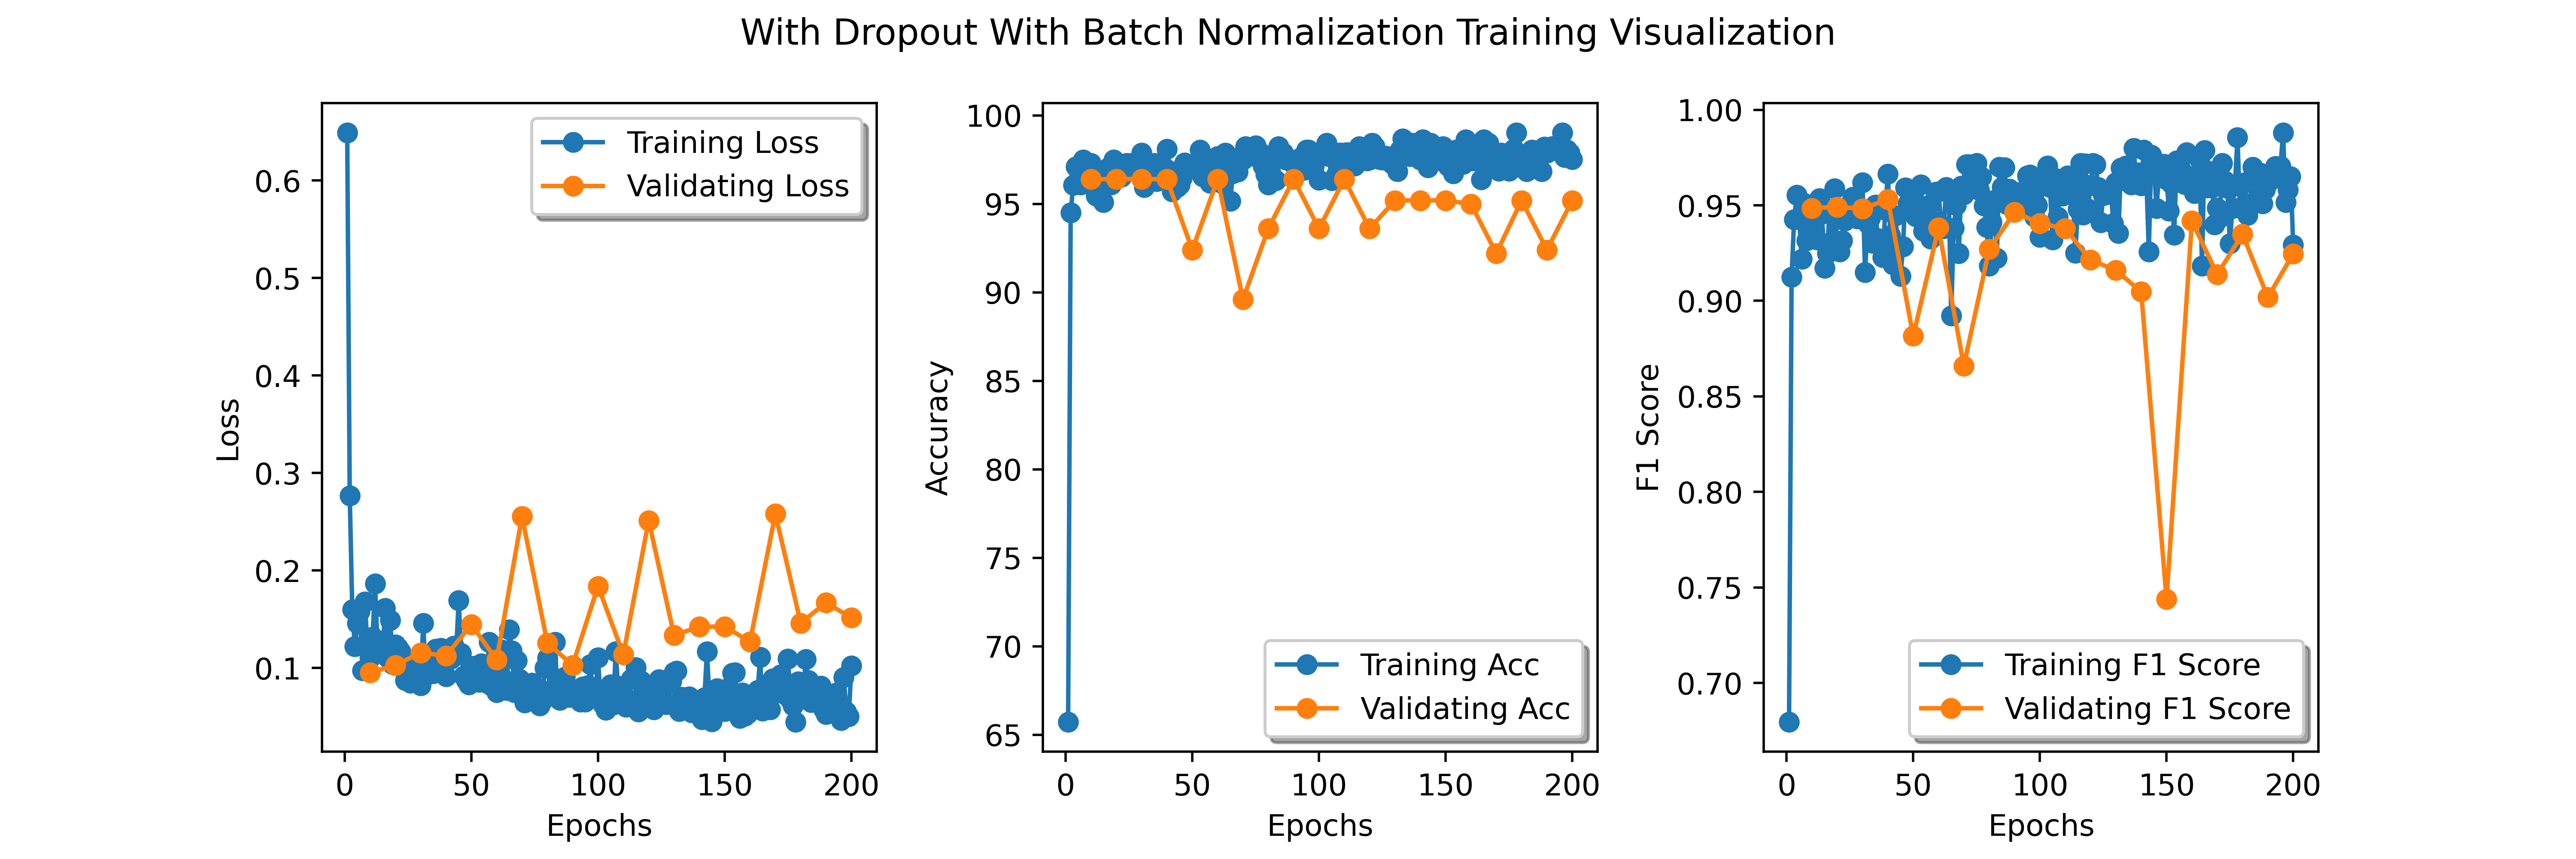
\includegraphics[width=1\textwidth]{Dropout_Batch_Normalization_64hn_3hl_200epochs_model.png}
\caption{Training Visualization for model with 3 hidden layers and 64 nodes for each hidden layer with Dropout and Batch Normalization}
\label{6}
\end{figure}\\

Now the model seems not overfitting anymore and the training loss and validation loss curves are closer to each other. The test result is listed below:

\begin{center}
   \begin{tabularx}{1\textwidth}{| >{\centering\arraybackslash}X | >{\centering\arraybackslash}X|>{\centering\arraybackslash}X|>{\centering\arraybackslash}X|}
\hline
   Accuracy & Precision & Recall & F1 Score\\
   \hline
     96.444 & 0.9310344827586207 & 0.9818181818181818 & 0.9557522123893805\\
     \hline
\end{tabularx} 
\end{center}

The confusion matrix is:
\begin{center}
    \begin{tabular}{|c|c|}
    \hline
    True Positive & False Negative \\\hline
        54 & 1 \\\hline
        4  & 82\\\hline
        False Positive & True Negative\\\hline
    \end{tabular}
\end{center}

However, no matter how hard we tried to tune the parameters or alter the architecture of the neural networks, overfitting problem can never be completely solved. Then can we use the best model in the training process selected by some criterion instead of the last model in the last epoch? Thus, I selected the model with least validation loss as the final model and retrain the whole network. The training process is below:
\begin{figure}[h]
\centering
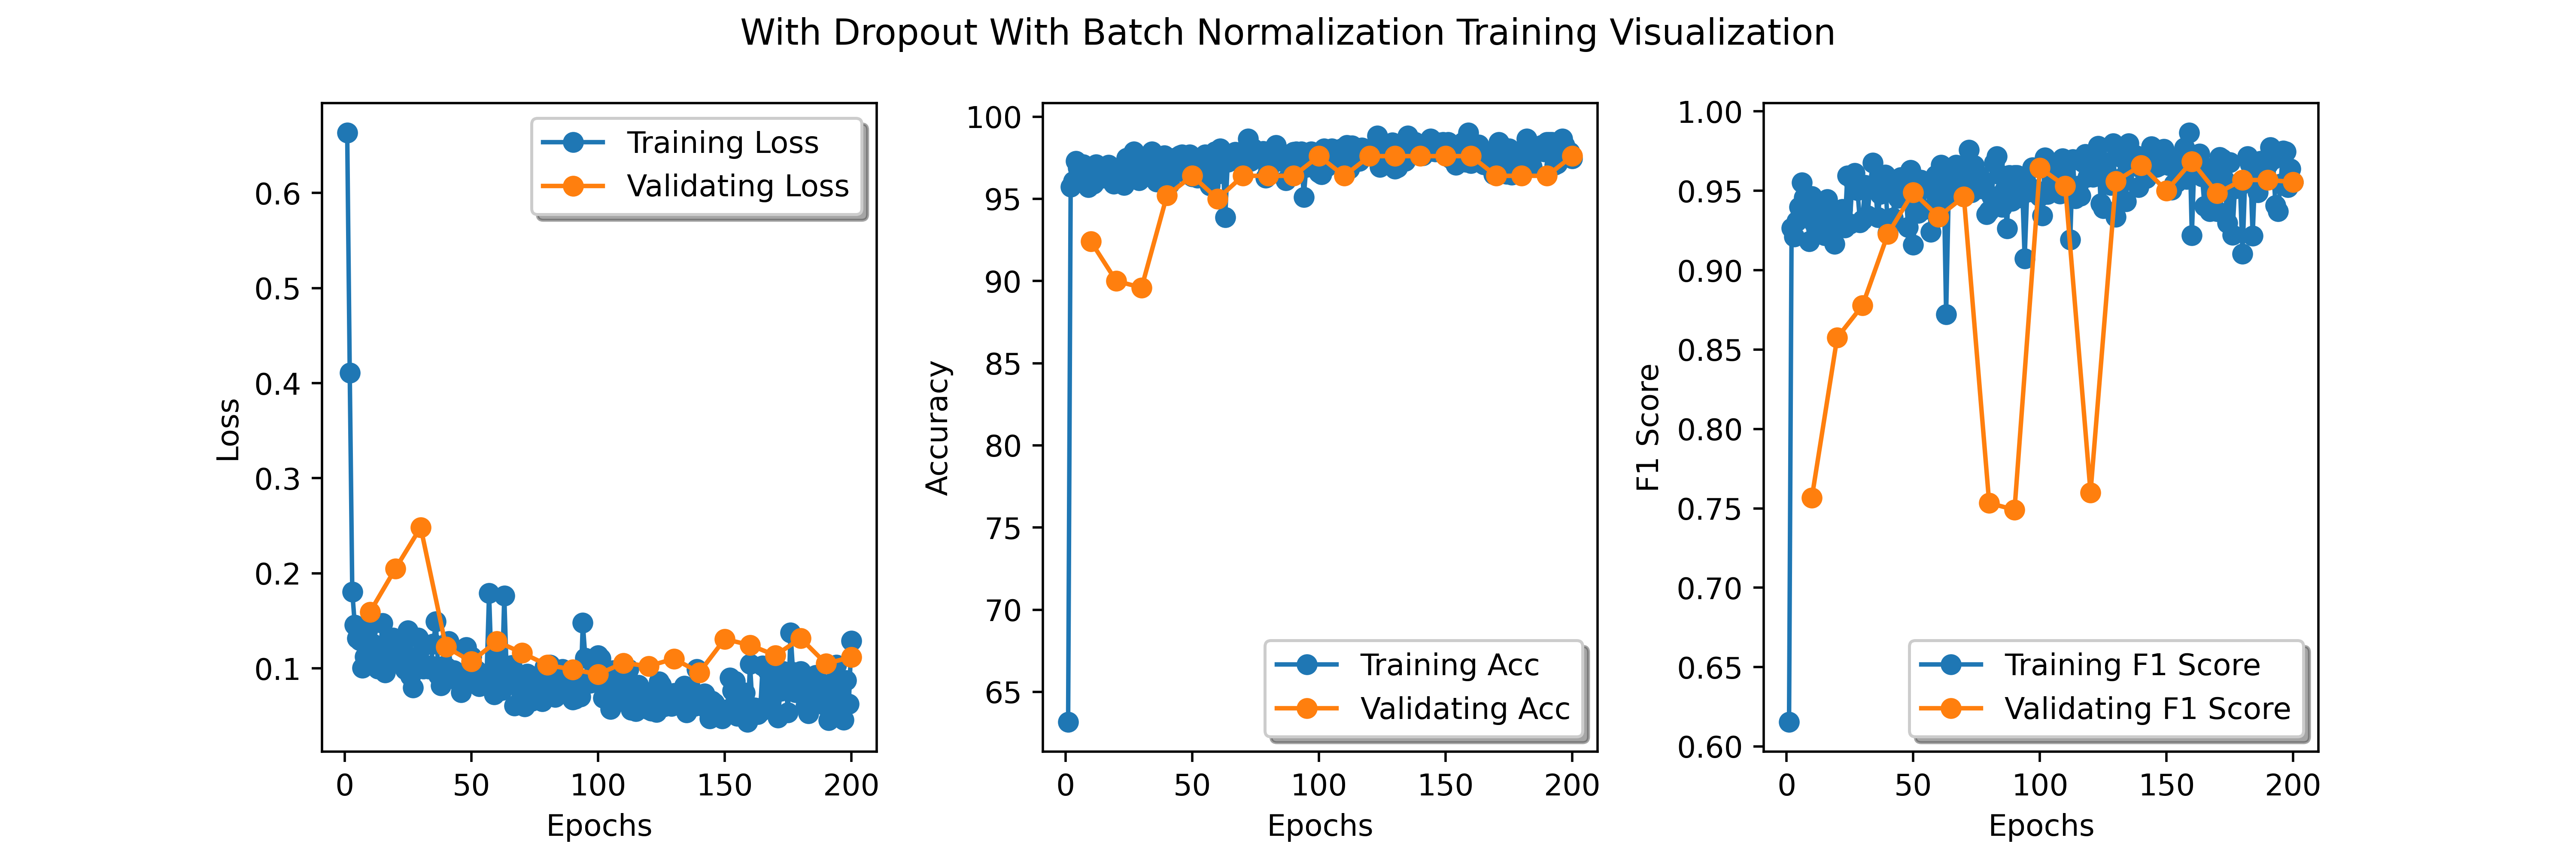
\includegraphics[width=1\textwidth]{loss_Dropout_Batch_Normalization_64hn_3hl_200epochs_model.png}
\caption{Training Visualization for model with 3 hidden layers and 64 nodes for each hidden layer with Dropout, Batch Normalization and Model Selection}
\label{7}
\end{figure}\\

The model still seems fine. The test result is listed below:

\begin{center}
   \begin{tabularx}{1\textwidth}{| >{\centering\arraybackslash}X | >{\centering\arraybackslash}X|>{\centering\arraybackslash}X|>{\centering\arraybackslash}X|}
\hline
   Accuracy & Precision & Recall & F1 Score\\
   \hline
     96.444 & 0.9464285714285714 & 0.9636363636363636 & 0.9549549549549549\\
     \hline
\end{tabularx} 
\end{center}

The confusion matrix is:
\begin{center}
    \begin{tabular}{|c|c|}
    \hline
    True Positive & False Negative \\\hline
        53 & 2 \\\hline
        3  & 83\\\hline
        False Positive & True Negative\\\hline
    \end{tabular}
\end{center}
The result is not getting better. The reason here might be that I should not use validation loss as the criterion since validation loss can never know if the model achieves the best performance on the validation set while precision, recall and F1 score are the most important keys to know if a binary classifier is good or bad. As a result, I change the criterion for model selection to F1 Score for each epoch. And for this time, the test result became a little bit better:
\begin{center}
   \begin{tabularx}{1\textwidth}{| >{\centering\arraybackslash}X | >{\centering\arraybackslash}X|>{\centering\arraybackslash}X|>{\centering\arraybackslash}X|}
\hline
   Accuracy & Precision & Recall & F1 Score\\
   \hline
     97.333 & 0.9473684210526315 & 0.9818181818181818 & 0.9642857142857142\\
     \hline
\end{tabularx} 
\end{center}

The confusion matrix is:
\begin{center}
    \begin{tabular}{|c|c|}
    \hline
    True Positive & False Negative \\\hline
        54 & 1 \\\hline
        3  & 83\\\hline
        False Positive & True Negative\\\hline
    \end{tabular}
\end{center}
Till now, I have achieved the best performance in all these attempts. However, a thought emerged in my mind: If the dataset seems not so complicated and the model is suffering from overfitting and covariant shift, why don't I just use a smaller network and larger batch size. Thus I modified the batch size to 64 and condensed the network to only 1 hidden layer with 5 nodes, and I removed all the batch normalization and dropout. Still, I select the best model with highest F1 score on the validation set. Then, the training progress becomes:
\begin{figure}[h]
\centering
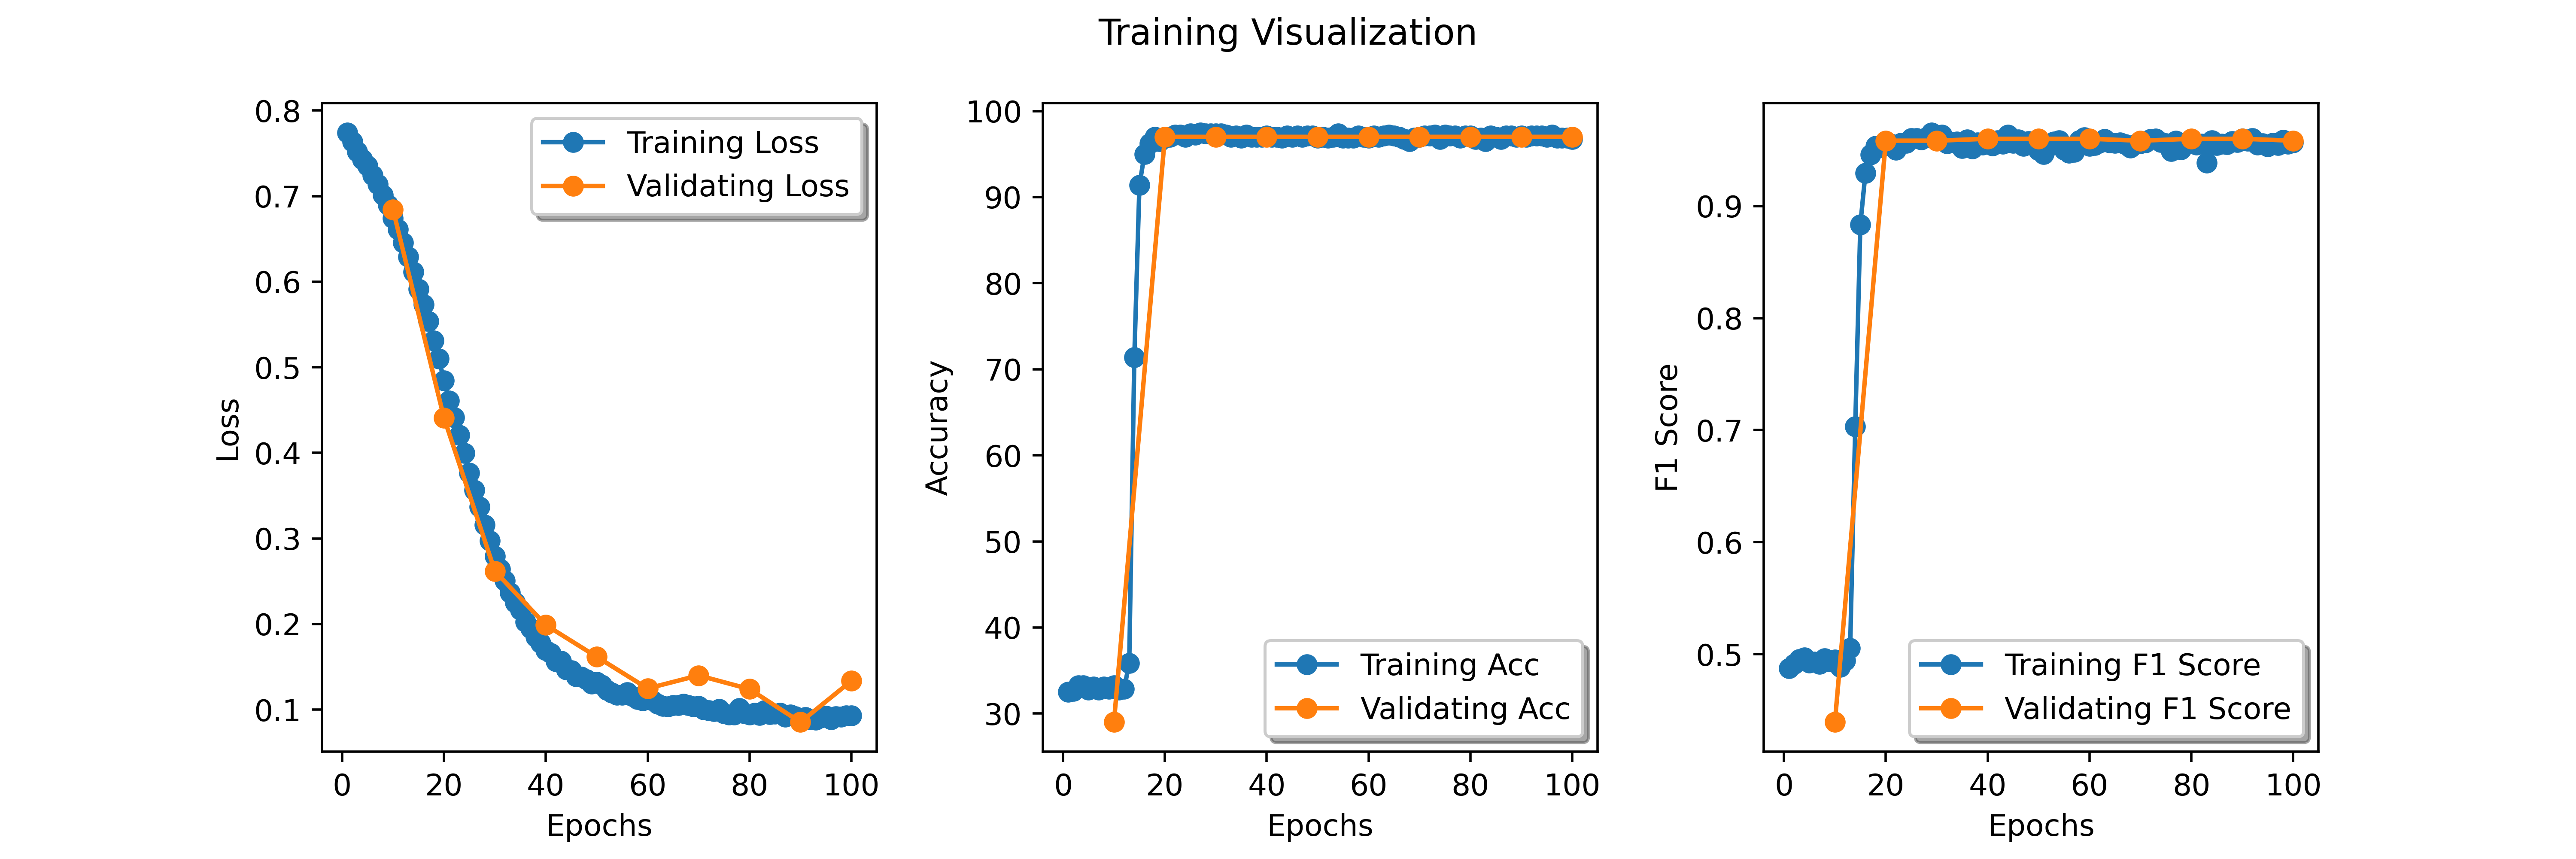
\includegraphics[width=1\textwidth]{8f1score_5hn_1hl_100epochs_model.png}
\caption{Training Visualization for model with 1 hidden layers with 5 nodes}
\label{8}
\end{figure}\\
Well... No overfitting, no covariant shift. Everything seems just fine. And the test result is:
\begin{center}
   \begin{tabularx}{1\textwidth}{| >{\centering\arraybackslash}X | >{\centering\arraybackslash}X|>{\centering\arraybackslash}X|>{\centering\arraybackslash}X|}
\hline
   Accuracy & Precision & Recall & F1 Score\\
   \hline
     97.333 & 0.9464285714285714 & 0.9636363636363636 & 0.9549549549549549\\
     \hline
\end{tabularx} 
\end{center}

The confusion matrix is:
\begin{center}
    \begin{tabular}{|c|c|}
    \hline
    True Positive & False Negative \\\hline
        53 & 2 \\\hline
        3  & 83\\\hline
        False Positive & True Negative\\\hline
    \end{tabular}
\end{center}
The result is as good as almost the best version from all larger models. Then I realized that, sometimes the best trick is no trick...
\end{document}
